\chapter{Order and object traces}
\label{sec:traces}

The extraction uses two traces (sites, orders and reduction names as defined in the Conventions, p.~\pageref{sec:conventions}). The
\emph{order trace} gives the position and curvature of each order on the detector. It defines the slit coordinate
$y_{\rm order}$ after the order is straightened (rectified), the region used for the sky, and the extraction window.
The \emph{object trace} $c(\lambda)$ gives the position of the object along the slit as a function of wavelength.
The optimal extraction weights each pixel by a spatial profile centred on the object trace. If the trace is wrong by
$d$ pixels and the profile is a Gaussian of standard deviation $\sigma$ pixels (here $\sigma$ is the profile width,
not an uncertainty), the extracted flux is biased by
\begin{equation}
\frac{F_{\rm est}}{F}=\frac{\sum_y P(y-d)\,P(y)}{\sum_y P(y)^2}=\exp\!\left(-\frac{d^2}{4\sigma^2}\right),
\label{eq:tracebias}
\end{equation}
i.e. a loss of 0.25--0.7 per cent for $d=0.5$\,px and $\sigma=5$--3\,px, but 6 per cent for $d=1.5$\,px and
$\sigma=3$\,px. Trace errors are largest at the faint ends of the orders, so the loss depends on wavelength. It
therefore does not cancel when the RM spectra are scaled to a common flux level (inter-calibration), which corrects
only a constant factor per spectrum. Fainter targets are the most exposed, because their traces are the least
well measured (Fig.~\ref{fig:trace_snr}).

\section{How \banzai{} traces the orders}
\label{sec:traces_orders}
\banzai{} fits the order shape once per slit width and instrument configuration, on a sky flat. The sky flats are
listed in a file distributed with the code (\texttt{data/orders/skyflats.dat}); for COJ after 2025 December 8 they are
the 2 and 6\,arcsec sky flats of that night. The pipeline stage that loads the order shape accepts no other type of
calibration frame, so data cannot be reduced without these sky flats. For each science frame, \banzai{} fits only a
shift of the orders along the slit ($y$), using a matched filter on the red order of the science frame itself, and
applies the same shift to both orders. The shift is stored in the header keyword \texttt{ORDYSHFT}.

To check this, we traced both orders on all 133 raw lamp flats of the campaign with the same \banzai{} tracing code
(Fig.~\ref{fig:order_lampflat}). The red order is traced over its full length at a signal-to-noise ratio of 900--2600
per column. Its shape agrees with that of the sky flat, taken about a year earlier, to 0.4\,px rms: the shape of the
orders has not changed. The blue order can only be traced at $x>1300$, where it agrees with the sky flat to
0.5--1.3\,px. At smaller $x$ the lamp is too faint (signal-to-noise ratio $\lesssim150$ per column) and the trace
wanders off. The position of the orders along the slit, in contrast, moves by $-2$ to $+4$\,px from block to block.
For the 6\,arcsec Fairall~9 blocks, the shift measured on the lamp flat of the same block agrees with
\texttt{ORDYSHFT} to 0.14\,px rms (mean difference $-0.30$\,px), so the archive order positions are correct for this
bright target. For a faint target the matched filter on the science frame has little signal, while the lamp flat is
equally bright for every target. Since every block includes a lamp flat, measuring the shift on it is the more robust
choice.

\begin{figure}[!htbp]
\centering
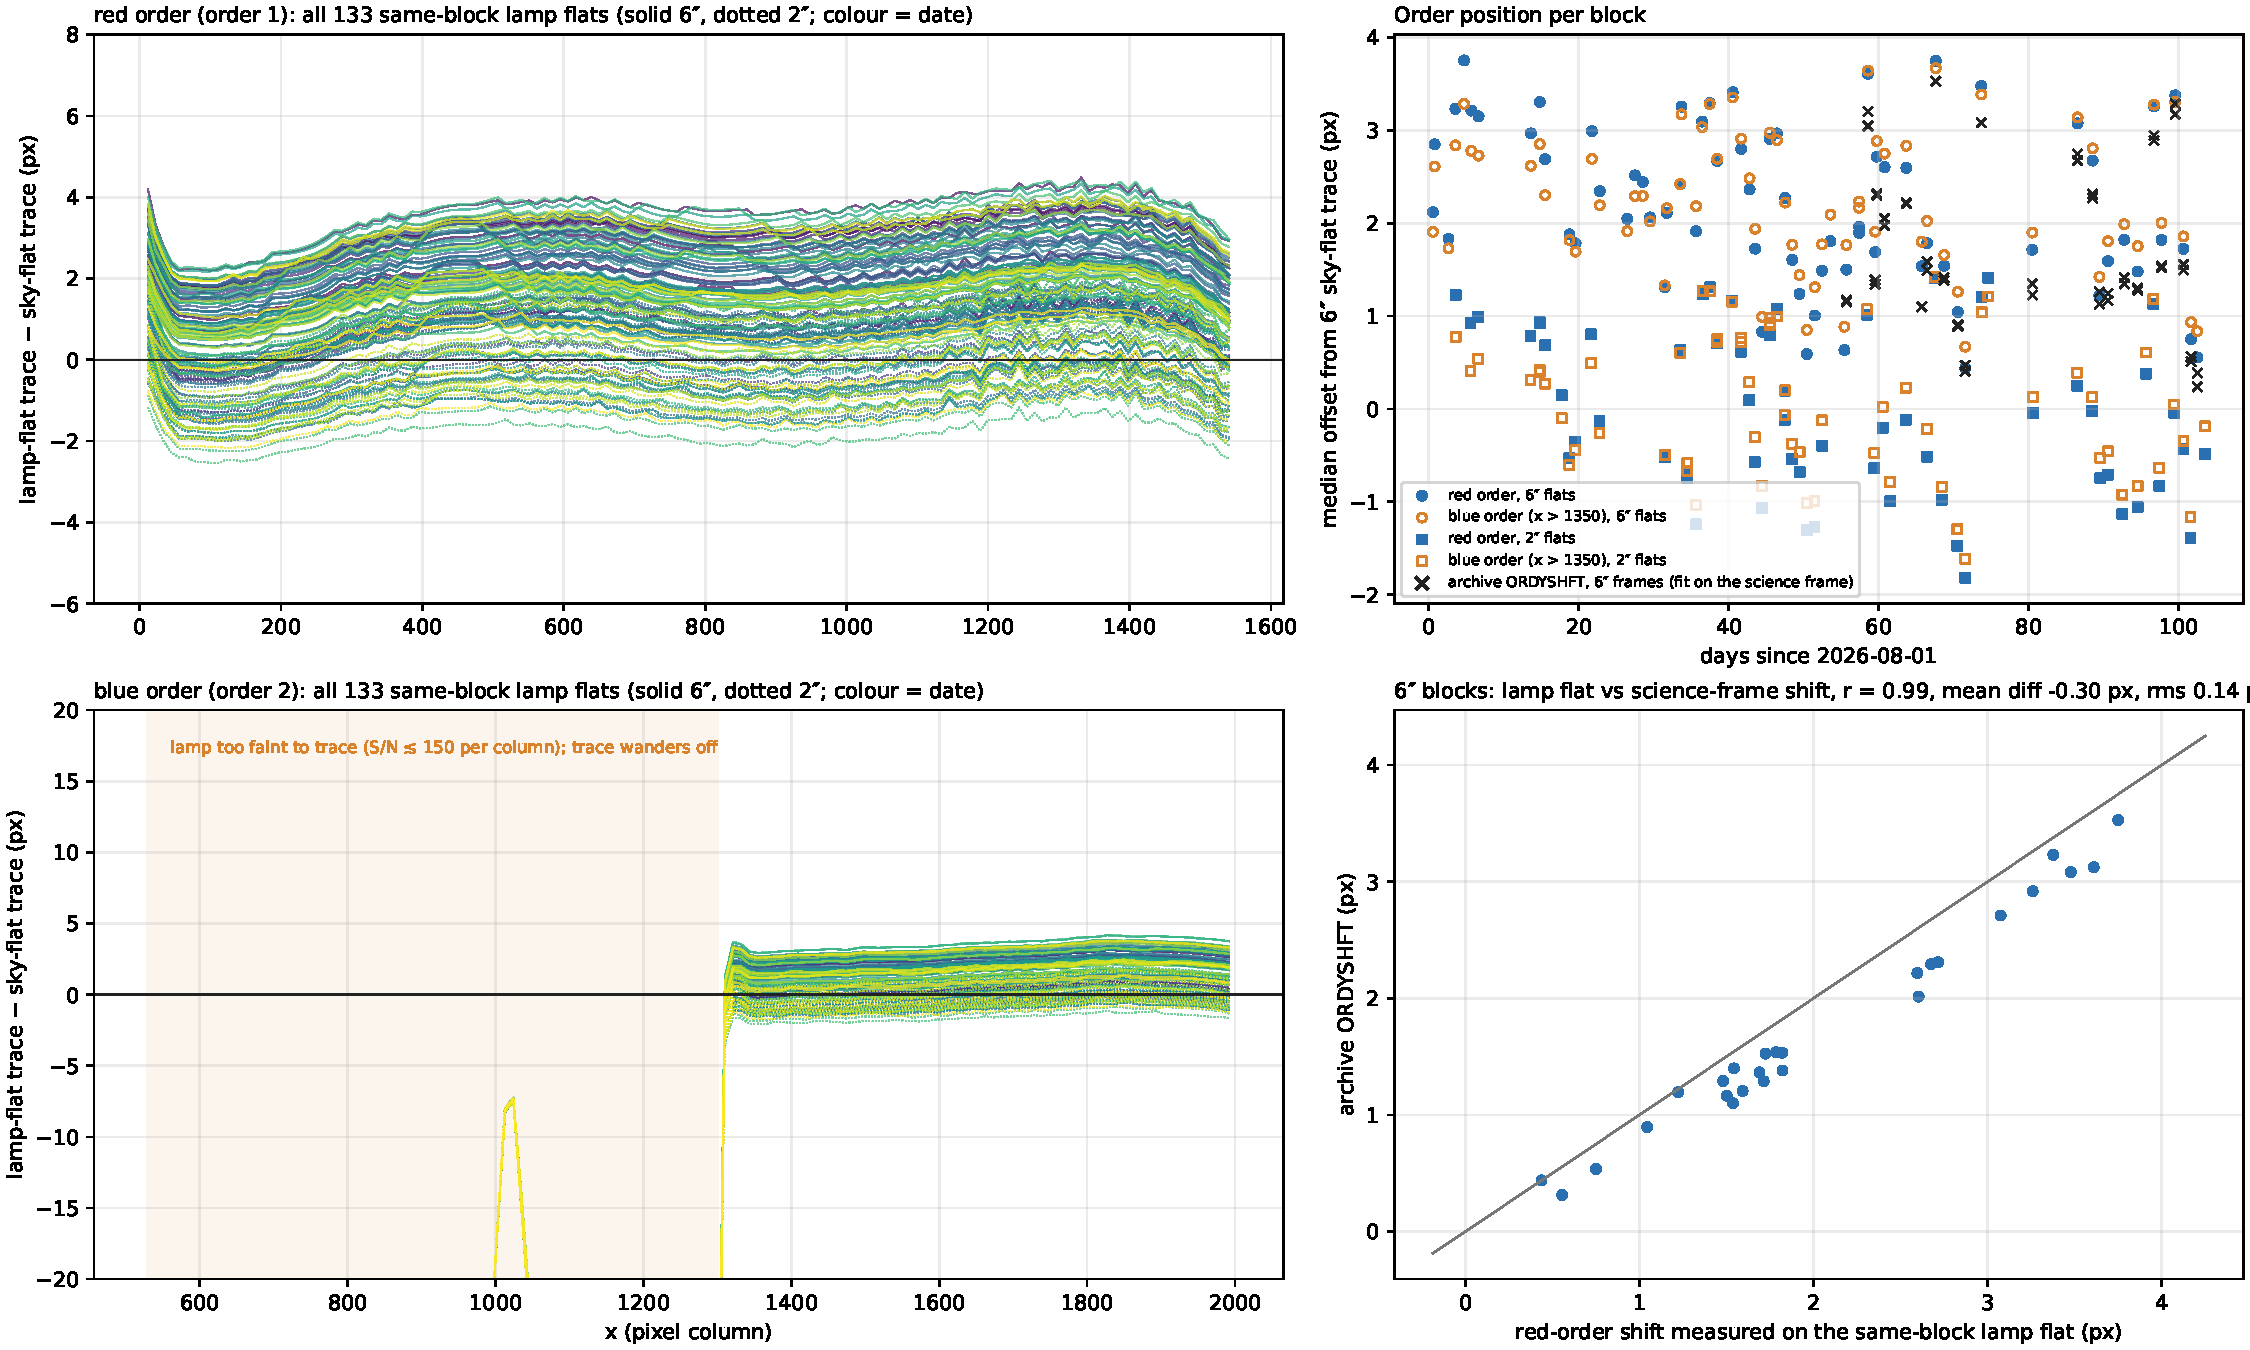
\includegraphics[width=\textwidth]{figures/fig_order_lampflat.pdf}
\caption{Position of the red order relative to the sky-flat trace. Left: shift measured on each of the 133 raw
lamp flats (filled: 6\,arcsec slit, open: 2\,arcsec) and the archive \texttt{ORDYSHFT} of the 6\,arcsec science
frames (crosses), against date. Right: for the 6\,arcsec blocks, the lamp-flat shift against \texttt{ORDYSHFT} of
the same block.}
\label{fig:order_lampflat}
\end{figure}

\section{How \banzai{} traces the object}
\label{sec:traces_object}
\banzai{} first finds the object in the spatial profile summed over all wavelengths. It then follows the object along
the dispersion in short wavelength intervals (\emph{chunks}): in each chunk the spatial profile is summed and the
centroid of its peak measured, and a polynomial in wavelength is fitted through the chunk centroids.
\banzai{}~1.0.1 used a single degree-7 polynomial over the whole order. \banzai{}~1.1.0 uses degree 5 with a penalty
on the second derivative, a minimum signal-to-noise ratio for each chunk and a limit on the jump between chunks.

\textit{Measurement.} We measured the object centroid independently on all 68 archive frames (50 of Fairall~9, 18
of EG\,21). In chunks of 100\,\AA{} (red order) and 50\,\AA{} (blue order), we collapsed the pixels of the
\texttt{BINNED2D} pixel table of the 2-d product (Section~\ref{sec:data}) onto $y_{\rm order}$ and fitted a Gaussian
plus a linear sky. Two problems of the archive data had to be handled. First, the \banzai{}~1.0.1 background is badly
wrong in the red order at 5200--5800\,\AA{} (it swings between $-360$ and $+950$\,counts), so we fitted our own sky.
Second, in some frames \banzai{}~1.0.1 divided the data by the invalid edge of a shifted lamp flat
(Chapter~\ref{sec:fringe}), which destroyed those pixels. They are not masked, but carry data $\approx0$ with an
uncertainty of $\approx10^{-4}$, so they dominate any inverse-variance weighting. We therefore dropped pixels whose
uncertainty is below 10 per cent of the median in the chunk. Neither the re-extraction of the archive products
(improved v1, Appendix~\ref{sec:app_v1}) nor the reduction from raw has such pixels.

Fig.~\ref{fig:trace_frame} shows a typical frame: the trace follows the object at both ends and in the middle of both
orders. The bright-moon frame of Fig.~\ref{fig:trace_frame_moon} shows the striped region destroyed by the flat
division at $x\approx210$--420 in the red order. On this pair of exposures our centroids appear offset from the trace
by 3\,px at 5350--5850\,\AA{}, which appears as the off-scale 6.7 per cent ``loss'' of the worst Fairall~9 frame in
Fig.~\ref{fig:trace_overview}. This offset is caused by the destroyed pixels, not by an error of the trace.

\begin{figure}[!htbp]
\centering
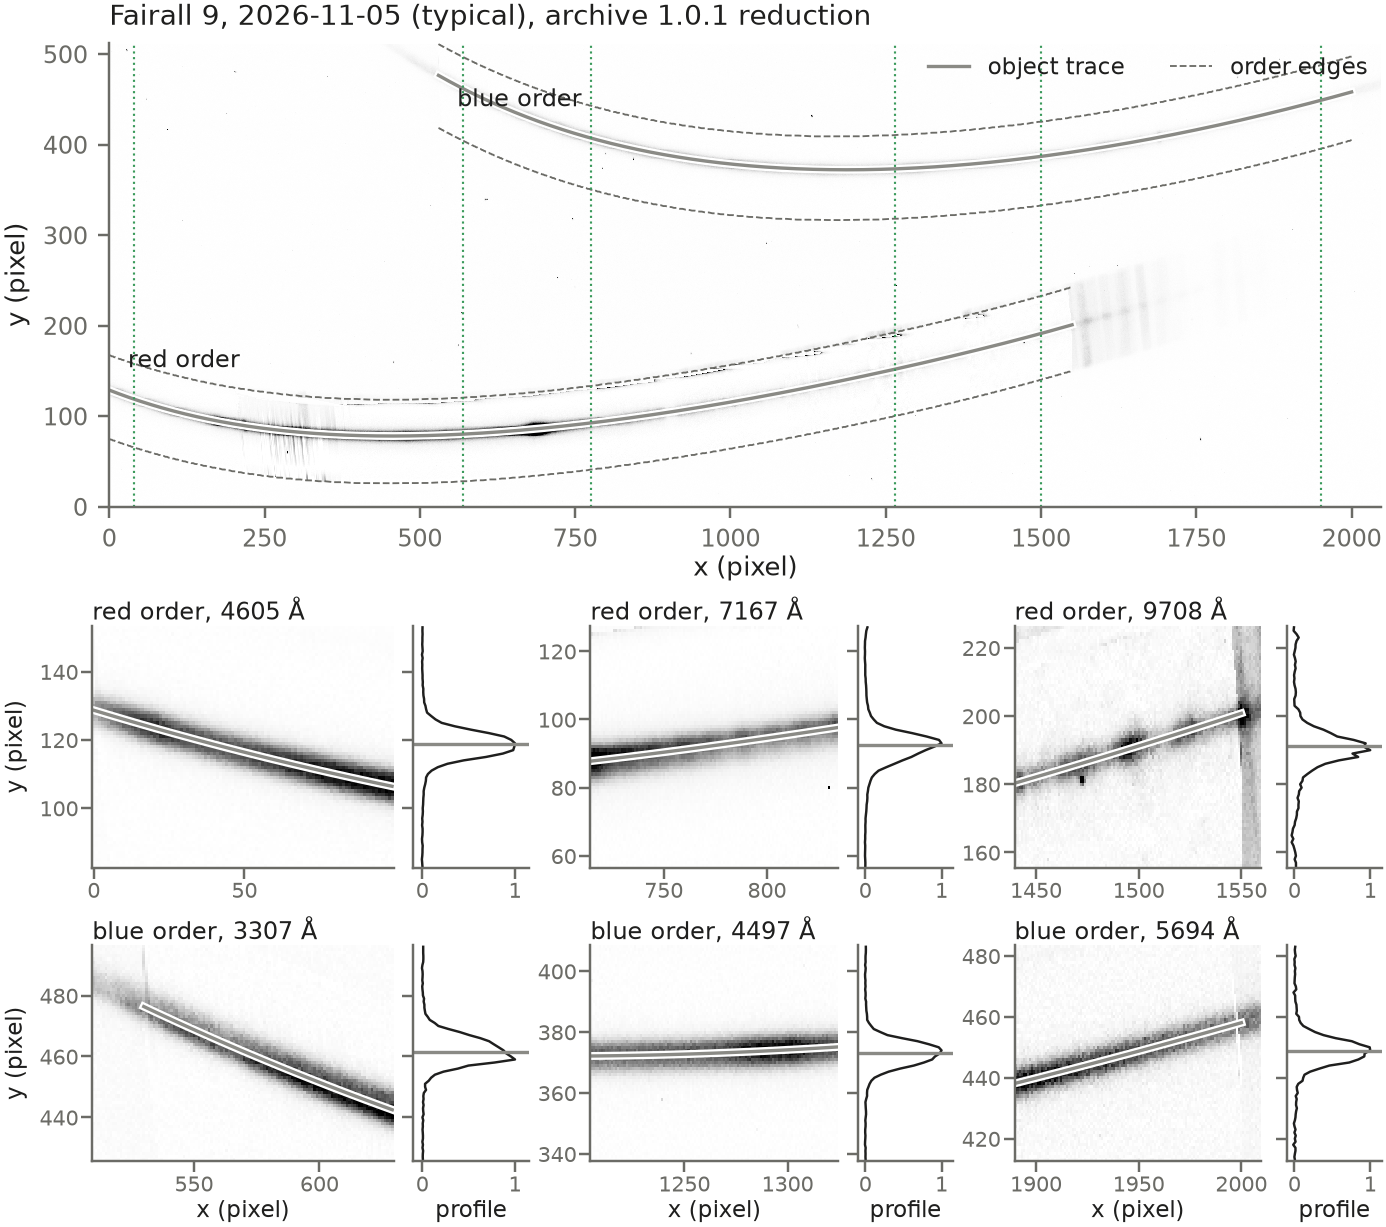
\includegraphics[width=\textwidth]{figures/fig_trace_frame_typical.png}
\caption{Fairall~9, 2026-11-05: background-subtracted archive frame with the order edges (dashed) and the
\banzai{}~1.0.1 object trace (grey with a white outline). The six zooms (green dotted lines) are at the two ends and
the middle of each order; next to each, the spatial profile (median over $\pm12$ columns) with the trace position.}
\label{fig:trace_frame}
\end{figure}

\begin{figure}[!htbp]
\centering
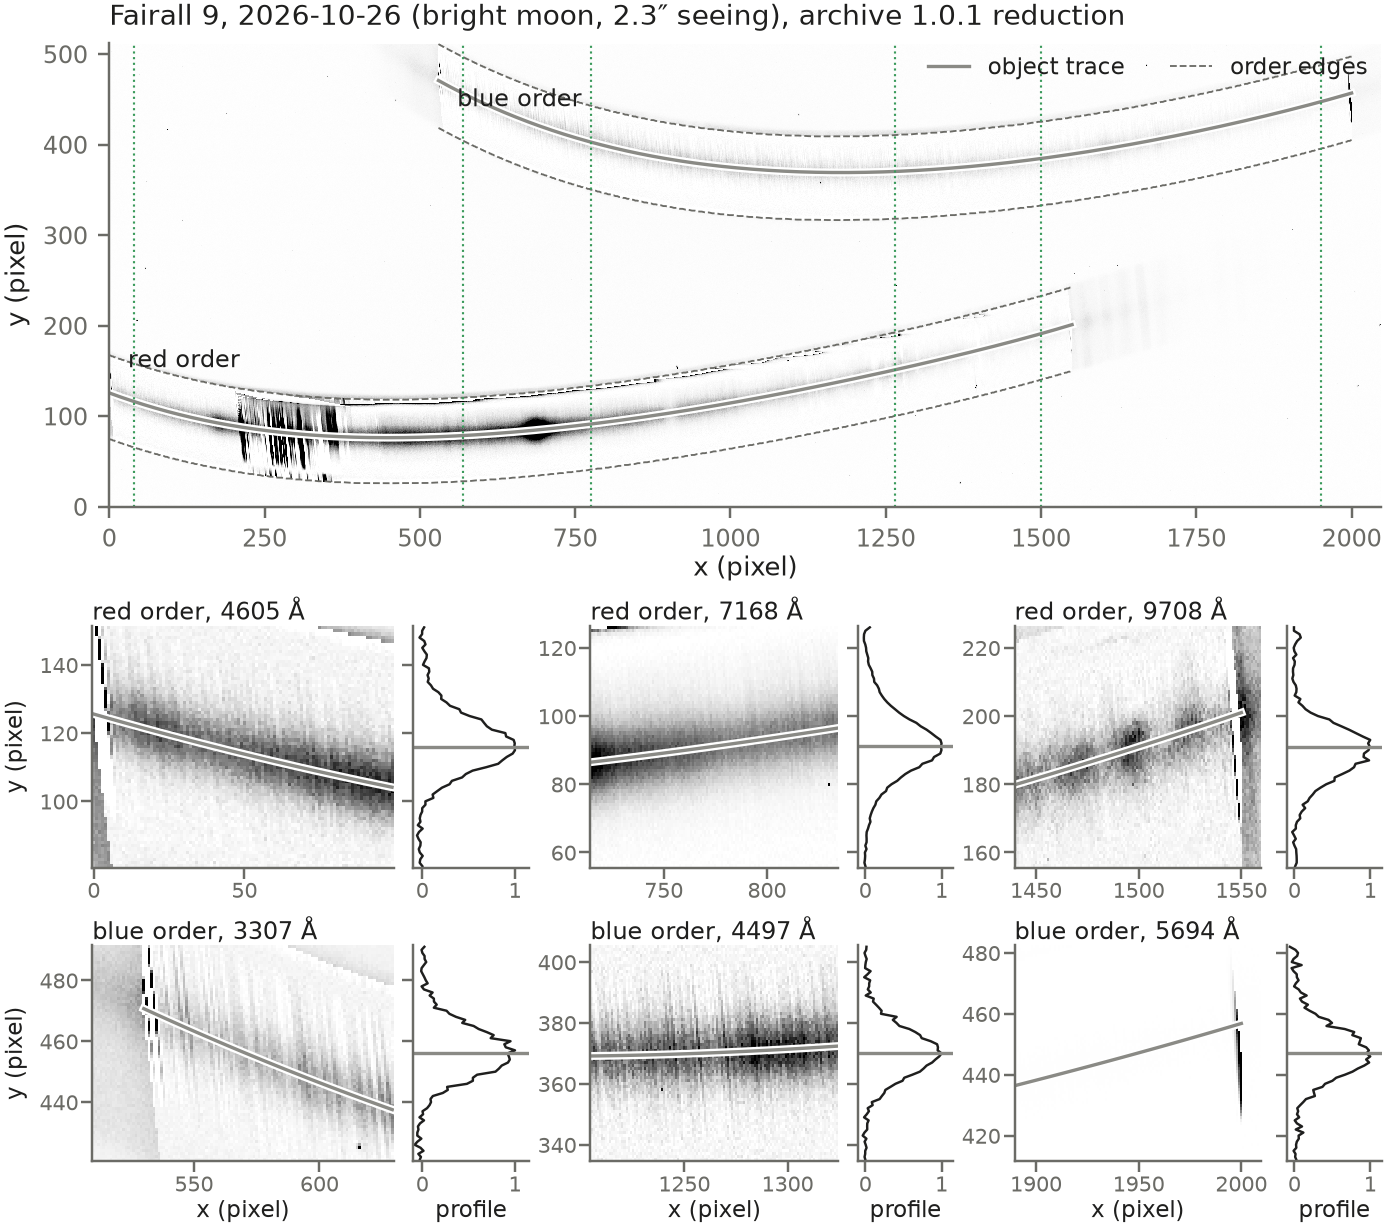
\includegraphics[width=\textwidth]{figures/fig_trace_frame_moon.png}
\caption{As Fig.~\ref{fig:trace_frame} for the bright-moon frame 2026-10-26 \#13 (2.3\,arcsec seeing). The striped
block at $x\approx210$--420 in the red order is where \banzai{}~1.0.1 divided by the invalid edge of the shifted
lamp flat.}
\label{fig:trace_frame_moon}
\end{figure}

\textit{Result.} The median offset between the measured centroid and the archive trace is 0.03\,px, and the flux loss
(eq.~\ref{eq:tracebias}) is below 0.1 per cent at nearly every wavelength (Fig.~\ref{fig:trace_overview}). The
exception is the faint red end, 9250--9750\,\AA. There the offsets reach 0.8--1.4\,px and the loss 1--2 per cent on
the worst frames, because the signal-to-noise ratio per chunk falls to 60--170 and the degree-7 polynomial is barely
constrained. These large offsets are much larger than the noise of the centroids (Fig.~\ref{fig:trace_snr}): they
come from the polynomial, which is poorly constrained at the ends of the fitted range.

\begin{figure}[!htbp]
\centering
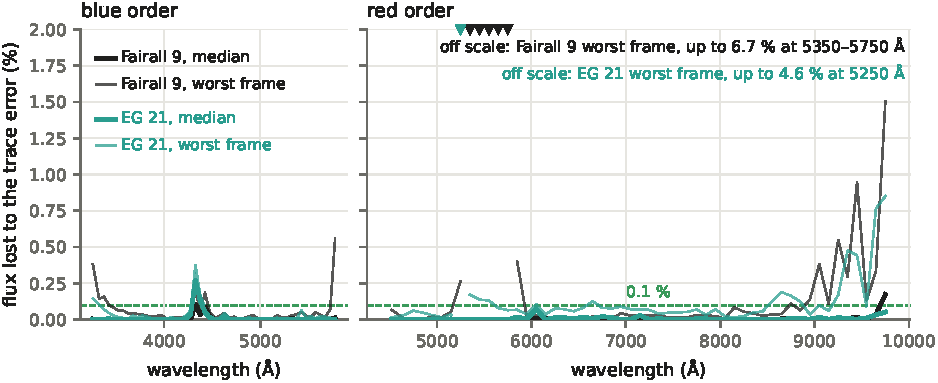
\includegraphics[width=\textwidth]{figures/fig_trace_overview.pdf}
\caption{Flux lost by the optimal extraction because of the error of the archive (1.0.1) object trace
(eq.~\ref{eq:tracebias}), per chunk: median (thick) and worst frame (thin) of the Fairall~9 and EG\,21 archive
frames. Dashed line: 0.1 per cent. Values above the axis are marked at the top edge with their peak value.}
\label{fig:trace_overview}
\end{figure}

\begin{figure}[!htbp]
\centering
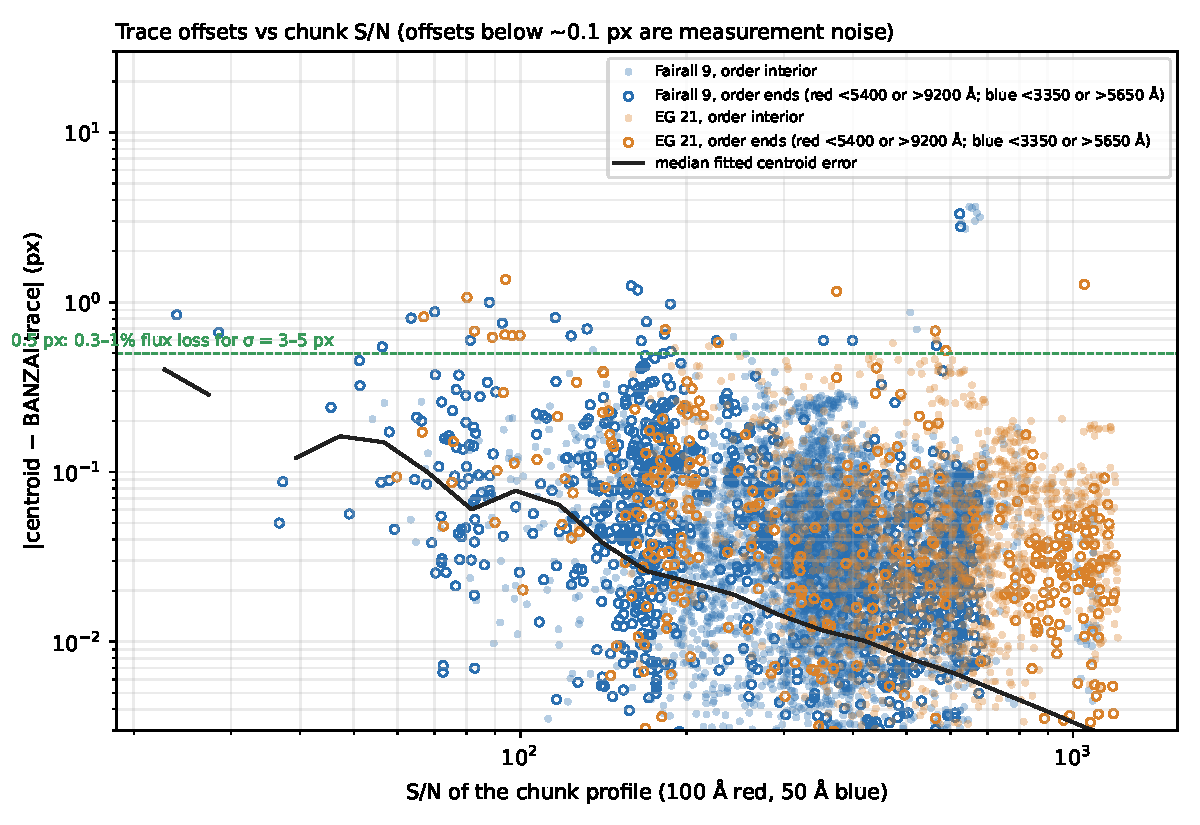
\includegraphics[width=0.75\textwidth]{figures/fig_trace_snr.pdf}
\caption{Absolute trace offset against the signal-to-noise ratio of the chunk; open symbols are chunks at the order
ends. Offsets below $\approx0.1$\,px are measurement noise (black line: median fitted centroid error).}
\label{fig:trace_snr}
\end{figure}

\section{A physical model of the object trace}
\label{sec:traces_model}
FLOYDS observes with the slit along the parallactic angle (rotator mode `vertical float', header keyword
\texttt{ROTMODE = VFLOAT}). Atmospheric differential refraction therefore moves the object \emph{along} the slit, by
\begin{equation}
\Delta y_{\rm ADR}(\lambda)=\frac{206\,265''}{0.337''}\,\left[n(\lambda)-n(\lambda_0)\right]\tan z ,
\label{eq:adr}
\end{equation}
with $n(\lambda)$ the refractive index of moist air at the measured pressure, temperature and humidity
\citep[the formulae collected by][]{Filippenko1982}, $\lambda_0$ a reference wavelength, $z$ the zenith distance, and
0.337\,arcsec the size of a pixel along the slit. For these frames the difference in position between 3300 and
9800\,\AA{} is 3.8--11.3\,px (median 5.9\,px). We model the object trace as
\begin{equation}
c(\lambda)=c_o+a\,\Delta y_{\rm ADR}(\lambda)+S_o(\lambda),
\label{eq:tracemodel}
\end{equation}
where $c_o$ is the position of the object in order $o$, $a$ scales the refraction, and $S_o(\lambda)$ is a fixed
instrumental shape per order (the part of the trace not described by refraction, e.g. the residual between the
order rectification and the true slit image), measured once on bright standards. Only three numbers are fitted per
frame ($c_1$, $c_2$ and $a$), with Gaussian priors on $c_1-c_2$ and $a$ (values below). We call this the
\emph{physical model}.

In our improved pipeline (improved v2 and v3) the physical model is combined with a correction $R_o(\lambda)$ fitted
to its residuals: a Legendre series of degree 5 with a penalty on its slope, so that it goes flat where nothing is
measured. The result, which we call the \emph{combined model}, is
\begin{equation}
c(\lambda)=c_o+a\,\Delta y_{\rm ADR}(\lambda)+S_o(\lambda)+R_o(\lambda).
\label{eq:tracehybrid}
\end{equation}
Where the chunk centroids are good, $R_o$ follows the structure specific to the frame. Where they are sparse or
noisy, the penalty suppresses $R_o$ and the physical model takes over. The template $S_o$ and the priors
($c_1-c_2=-0.87\pm0.29$\,px, $a=0.58\pm0.14$) were measured on 38 standard-star frames of COJ reduced from raw
(Chapter~\ref{sec:raw}). $S_o$ is tabulated every 50\,\AA{} (red order) and 25\,\AA{} (blue order), smoothed over 5
points, and agrees with the median of the stacked standard-star traces to 0.01--0.02\,px. Its peak-to-peak amplitude
is $\approx1$\,px in both orders. The fitted $a$ is 0.4--0.7 rather than 1. We attribute this to the slit not being
exactly at the parallactic angle and to the order rectification absorbing part of the refraction. Since $a$ is
fitted, only the shape of $\Delta y_{\rm ADR}(\lambda)$ matters. The template and priors are specific to each
instrument: OGG has its own, built in the same way from 100 standard-star frames (Section~\ref{sec:sites_trace}).

\textit{Fainter targets.} To test the regime that matters for faint AGN, we simulated fainter versions of Fairall~9.
We took the chunk centroids that \banzai{}~1.1.0 measured on the 100 Fairall~9 exposures reduced from raw, and made
the target 3--100 times fainter: the centroid error of each chunk was scaled up, noise of that size added, and chunks
below the pipeline's detection threshold dropped. We then refitted the trace with the pipeline's own fitting
functions and compared it with the trace fitted to the original centroids, which we take as the truth
(Table~\ref{tab:tracefaint}). The 1.1.0 polynomial is good up to $\approx10$ times fainter than Fairall~9. At 30 times
fainter its error at the order ends grows to 0.8\,px (90th percentile), and at 60 times to 3.5\,px. The physical
model keeps the error at the ends to 0.3--0.4\,px down to 60 times fainter. The combined model
(eq.~\ref{eq:tracehybrid}) is the best or equal best at every level up to 30 times fainter, including the original
brightness (median error 0.06\,px at the ends, like the polynomial, and 0.03\,px in the interior). At 100 times
fainter most chunks fall below the detection threshold, and a fifth of the frames cannot be traced by any method.

\begin{table}[!htbp]
\centering
\caption{Error of the object trace for simulated fainter versions of the 100 Fairall~9 exposures, with the
pipeline's own fitting functions: median / 90th percentile of $|c_{\rm fit}-c_{\rm true}|$ in pixels in the
interior and at the ends of the orders (red $>9200$\,\AA; blue $<3400$ or $>5650$\,\AA). Frames that could not be
traced at all are not included (in brackets: their number).}
\label{tab:tracefaint}
\begin{tabular}{lcccccc}
\toprule
 & \multicolumn{2}{c}{Polynomial (1.1.0)} & \multicolumn{2}{c}{Physical (eq.~\ref{eq:tracemodel})} &
 \multicolumn{2}{c}{Combined (eq.~\ref{eq:tracehybrid})} \\
Fainter by & interior & ends & interior & ends & interior & ends \\
(factor) & (px) & (px) & (px) & (px) & (px) & (px) \\
\midrule
1 & 0.05 / 0.11 & 0.06 / 0.16 & 0.06 / 0.16 & 0.11 / 0.28 & 0.03 / 0.08 & 0.06 / 0.16 \\
10 & 0.05 / 0.12 & 0.10 / 0.27 & 0.06 / 0.17 & 0.12 / 0.30 & 0.03 / 0.09 & 0.08 / 0.21 \\
30 & 0.06 / 0.19 & 0.18 / 0.79 (1) & 0.07 / 0.21 & 0.13 / 0.32 & 0.05 / 0.16 & 0.12 / 0.34 \\
60 & 0.11 / 0.43 & 0.75 / 3.51 (6) & 0.09 / 0.28 & 0.15 / 0.38 (5) & 0.08 / 0.31 & 0.17 / 0.55 (5) \\
100 & 0.20 / 0.71 & 0.66 / 1.84 (19) & 0.17 / 0.58 & 0.24 / 0.65 (16) & 0.17 / 0.62 & 0.26 / 0.87 (16) \\
\bottomrule
\end{tabular}
\end{table}

\textit{On the real data.} The combined model is the default of improved v3 (pipeline setting
\texttt{PROFILE\_TRACE\_MODEL = 'adr'}). On the 157 frames reduced from raw (100 Fairall~9, 18 EG\,21, 39 Feige\,110),
its traces are slightly better than those of \banzai{}~1.1.0 (stock) in every measure (Table~\ref{tab:tracereal}).
The flux loss at the order ends (90th percentile) drops from 0.15--0.19 to 0.11--0.13 per cent. For bright targets
the trace was never a problem; the change matters for faint ones.
Fig.~\ref{fig:trace_compare} compares the archive and the improved v3 traces with the measured centroids on three
frames. On the typical frame the archive trace follows the centroids more closely than the improved v3 trace (rms 0.09
against 0.21\,px); the improved v3 trace departs by up to 0.7\,px at the blue end of the blue order. On the frame with a
faint red end, and on EG\,21, it is the other way round. There the archive polynomial bends away beyond 9600\,\AA{}
(by up to 0.9 and 1.4\,px respectively), while the improved v3 trace stays within 0.8\,px everywhere. The rms of the
archive and improved v3 traces are 0.20 and 0.17\,px on the faint-red-end frame, and 0.36 and 0.24\,px on EG\,21.

\begin{table}[!htbp]
\centering
\caption{Trace offsets on the frames reduced from raw: measured centroid minus trace, median / 90th percentile
(pixels), and the 90th percentile of the flux loss at the order ends.}
\label{tab:tracereal}
\begin{tabular}{llccc}
\toprule
Frames & Trace & interior & ends & loss at ends \\
 & & (px) & (px) & (\%) \\
\midrule
Fairall~9 (100) & 1.1.0 polynomial & 0.075 / 0.22 & 0.10 / 0.37 & 0.15 \\
 & combined model & 0.064 / 0.21 & 0.09 / 0.30 & 0.11 \\
EG\,21 (18) & 1.1.0 polynomial & 0.074 / 0.23 & 0.10 / 0.43 & 0.19 \\
 & combined model & 0.060 / 0.22 & 0.08 / 0.33 & 0.11 \\
Feige\,110 (39) & 1.1.0 polynomial & 0.077 / 0.25 & 0.10 / 0.42 & 0.19 \\
 & combined model & 0.063 / 0.25 & 0.08 / 0.35 & 0.13 \\
\bottomrule
\end{tabular}
\end{table}

\begin{figure}[!htbp]
\centering
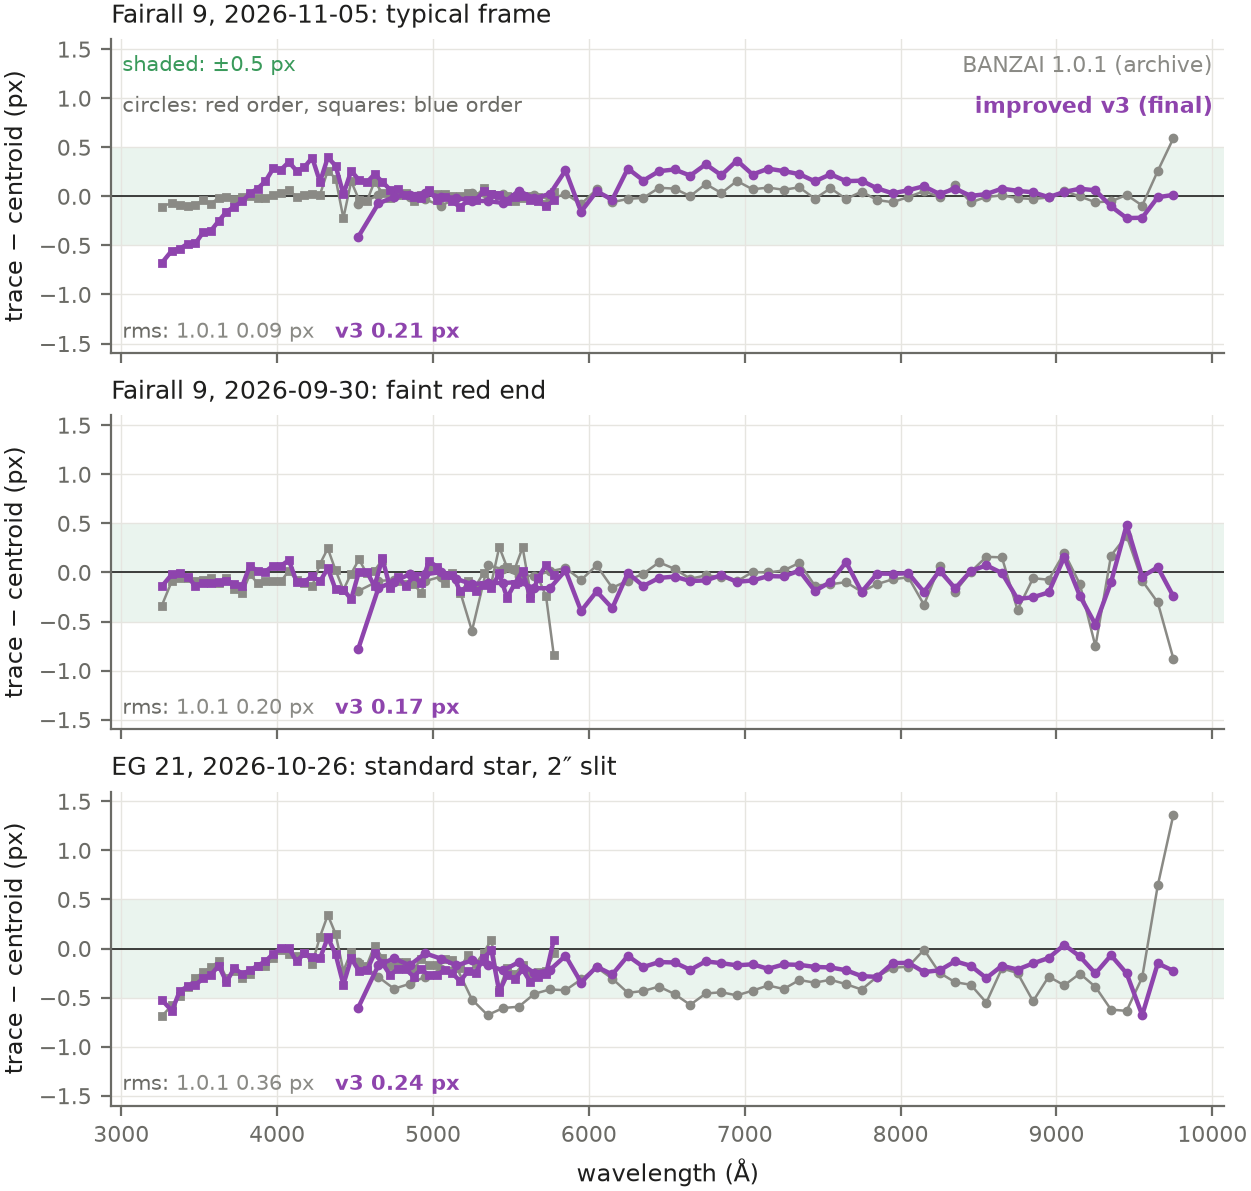
\includegraphics[width=\textwidth]{figures/fig_trace_compare_a.png}
\caption{Object trace minus measured centroid against wavelength for three frames: the archive \banzai{}~1.0.1
trace (grey) and the improved v3 trace (purple, combined model); circles red order, squares blue order; shaded
$\pm0.5$\,px. The archive trace is compared with centroids measured on the archive frame, the improved trace with
centroids measured on the same exposure reduced from raw. The rms over both orders is given in each panel. The
Gaussian centroids are offset by $\approx0.2$\,px from the matched-filter traces in parts of the red order because the
profile is not exactly Gaussian; only the variation with wavelength matters.}
\label{fig:trace_compare}
\end{figure}
